% !TEX root = ../main.tex


\section{Introductory Remarks}




decentralized exchanges allow the market participants to be fully authoritative over their assets using their private keys. 
One issue with decentralized 

Cryptocurrency trading on centralized exchanges has been shown to be vulnerable to cybersecurity hacking and internal frauds over the years, with the most infamous hacks being Mt. Gox and Coincheck. In addition, trading on centralized exchanges is not compatible with DeFi applications since it is technically infeasible to bridge between decentralized applications and centralized servers without compromising the trust model.


Digitex is the intelligent combination of the speed and reliability of centralized servers with the trustless security of decentralized smart contracts. The Digitex Futures Exchange interacts with the smart contract so that it can update a trader’s available balance to reflect that trader’s outstanding margin liabilities and his trading profits and losses, but the exchange does not have physical possession of the trader’s funds and is unable to do anything else to the funds held in the smart contract.
The






% = = = = = = = = = = = = = = = = = = = = = = = = = = = = = = = = = = = = = = = = = =

\section{Related Work}



% = = = = = = = = = = = = = = = = = = = = = = = = = = = = = = = = = = = = = = = = = =





% Discussed in the meetings:
% do the followings for the worst case matching:
%	1- Find the actual gas limit for the Ethereum blockchain and set the gas limit of ganache to that number
%	2- Try to find the actual gas cost before the refund for each PQ (and that number should be close to the gas limit). Have another column in the worst case matching table for that number

% Have one chart with all the worst case submission and one for random case submission 
% Increase the gas limit basically to the infinity and find the gas cost for matching 1000 orders (worst case matching). Why? because Ethereum might improve over the time and we'd like to know how would that affect each PQ in case of handling worst case matching. If you find a problem with Node.js we can just copy that error and discuss it inside the paper. In that chart, we can add horizontal lines for each gas limit (today, proposed, etc) (Ethereum (ETH) miners are currently voting to expand the block gas limit from 10,000,000 to 12,500,000 gas, according to a recent tweet from Bitfly, the parent company of Ethermine pool: https://cointelegraph.com/news/ethereum-miners-vote-to-increase-gas-limit-causing-community-debate)

% Deleting the unavailable mapping remains a challenging issue to solve (have a little section in the paper to discuss our different solutions for it). 
%	1- we can just create a new mapping everytime the market opens and have a modifier for the claim functions so that they could be called only when the market is closed. 
%	2- we can have custom keys for the mapping (like a counter we define as a global variable and increment it at the end of the match function). So everytime the new market starts, we just use another portion of the mapping.
%	3- we can have another smart contract which only stores the mapping and just delete that after the close function. 

% We use one-shot market for the sake of our performance tests on different datastructures. and once we have all the numbers we can think about iterated market.

% Our two competitors are Uinswap and Loopring (that uses ZK roll ups):
% 	1- Uniswap: we can argue that in traditional markets we have various traditional exchanges. Each of these exchanges have different trading rules and designs which work for different traders.
%	2- Loopring:
%		2-1: Barrier to entry: In order for a trader to trade specific ERC20 on Loopring, Loopring has to agree to support that token. It might not be difficult and they probably approve the token as long as it is standard compliant.
%		2-2: ZK proofs are quick and cheap to verify but they are expensive and time consuming to generate: (1) now they are generating these proofs for free but later they charge traders for doing that. (2) Looping does not probably generate these proofs per every block so the settlement and 				clearing is not happening per block. So we have faster clearing and settlement as we clear everything per block. 
% 		2-3: Loopring is non-custodial, meaning that the money moves only when the proofs come, so there is a latency in transferring funds to the traders.















Another important "limit" is that the gas refund is provided only 1 time, at the very end of the transaction's execution.
This means that a transaction cannot use its own gas refund to pay for any part of its execution.
A refund cannot be used to avoid Out of Gas exceptions








Executed orders are permanently deleted from the storage instantly. 



Deletion
Ethereum gives us a gas refund when we delete variables. Its purpose is an incentive to save space on the blockchain, we use it to reduce the gas cost of our transactions.
Deleting a variable refunds 15,000 gas up to a maximum of half the gas cost of the transaction. Deleting with the delete keyword is equivalent to assigning the initial value for the data type, such as 0 for integers.





Appendix G. Fee Schedule in the Yellow Paper-EIP-150, shows that a gas refund of 15,000 is given for each state slot that is set to zero. These refunds are calculated during execution but only paid back post-execution.
The Fee Schedule also states that changing a store from a Zero value costs 20,000 but changing a non-Zero store costs only 5000. The notable difference being the 15,000 refund.
So the net cost of a store and delete is 5000 gas. If the entire 20,000 gas or more was refunded, then there is effectively no net cost for storage operations and its IO overhead. A cheap attack could be launched by continuous store/delete.

heap-mapping with delete mapping (30 orders) : 3,111,416
heap-mapping without delete mapping (30 orders) : 3,582,291


You should be aware the refund is done at the end of the transaction, you have to have enough gas to process each slot upfront. Also your refund can be at most half of the gas used
Recall that the gas refund can give you up to half of your consumed gas back, so even in the best case, you won't actually break even.

GasToken works by taking advantage of the storage refund in Ethereum

Store data permanently on Ethereum is extremely expensive. It has no 

DApps on Ethereum execute arbitrary code provided by the owner of the DApp. While this code might be written
in a high-level programming language like Solidity, it is compiled to a compact representation (called ‘bytecode’)
that is a set of low-level instructions to the environment (Ethereum virtual machine or EVM). Because different
functions will have different complexities, the user running the function pays in proportion to the number of
instructions, the complexity of the instructions, and the storage requirements. This means that each operation has a fixed price. Naturally the operations might be priced in ETH, since it is the on-board currency, however this
would cause the price of computation to be as volatile as Ether itself. Instead, Ethereum uses a pseudo-currency
called gas.5 Each instruction has a fixed price in gas. A user who wants to run a function will offer to pay a certain
amount of ETH per unit of gas to the miner who finalizes the function. Miners will generally choose which
functions to run first based on how much ETH/gas they offer, and they might ignore functions that offer too little
ETH/gas. We describe gas as a pseudo-currency because it cannot be directly stored or transacted, however we
will revisit this below



The obvious is answer is that you can receive gas refunds for releasing unused storage. In the yellow paper on page 25 'Appendix G. Fee Schedule', you can read the gas costs for each instruction. As you might know, SSTORE will generally create the most costs in your contracts with a significant cost of 20,000 gas per instruction. On the contrary, if you look at %R_sclear:

Refund given when the storage value is set to zero from non-zero.

15,000 gas refund means you can actually get 75% of your storing costs back! That is a large amount, do not forget about this. And the solution is simple, just set a value back to 0 once you are sure it will not be used anymore.


Cost of a Transaction
The total cost of a transaction in the Ethereum network is based on two factors:
gasUsed is the total gas that is consumed
gasPrice specified in the transaction
<strong>Transaction Cost</strong>
Total Transaction Cost = gasUsed * gasPrice





The only two OPCODEs with negative gas costs are STORAGEKILL(-15000) and GSUICIDEREFUND(-24000).

These occur when storage values are deleted or contacts are suicided.

These OPCODEs grant gas refunds because they free up space in the blockchain.



Also, Solidity \textit{delete()} function does not 



Clearing Mappings

The Solidity type mapping (see Mapping Types) is a storage-only key-value data structure that does not keep track of the keys that were assigned a non-zero value. Because of that, cleaning a mapping without extra information about the written keys is not possible. (from : https://solidity.readthedocs.io/en/v0.5.12/security-considerations.html) So in order to wipe the unavailable Ether and token balances of all the market participants after matching is completed, we have to iterate over mapping using an array we use to store the mapping keys.





In short, the sender of the transaction that causes the storage location to be freed (set to zero) will have an amount (a net 10000 gas per freed storage location) deducted from the total amount of gas used for the transaction.

It's a bit more nuanced in reality:

The gas cost of setting the location to zero is 5000 %(G_sreset in the Yellow Paper).
15000 gas is added into the refund counter %(R_sclear in the Yellow Paper).
At the end of a successful transaction the amount of gas in the refund counter (up to a cap of half the total gas used) is added to the unused gas and returned to the caller (Eqn 72 in the Yellow Paper).
References above are to this version of the Yellow Paper, which discusses the Refund Counter in sections 6.1 and 6.2.

The gas price is whatever gas price applies to the whole transaction in which the refund occurs




delete a assigns the initial value for the type to a. I.e. for integers it is equivalent to a = 0, but it can also be used on arrays, where it assigns a dynamic array of length zero or a static array of the same length with all elements reset. For structs, it assigns a struct with all members reset.

delete has no effect on whole mappings (as the keys of mappings may be arbitrary and are generally unknown). So if you delete a struct, it will reset all members that are not mappings and also recurse into the members unless they are mappings. However, individual keys and what they map to can be deleted.











EIP-114, or the “1/64ths rule”
EIP-114 mandates that certain stackdepth-creating opcodes withhold 1/64th of remaining gas from the stack they create. In practice this means:
The gas required for a successful transaction can be greater than the actual gas spent (similar to how gas refunds behave).
The extra gas required for a successful transaction varies depending on the transaction’s initial gasamount.
A long-standing issue with Ganache has been the fact that we haven’t returned EIP-114 compliant gas estimations. This has caused our gas estimates to be too low in cases where a transaction executed certain opcodes. Gas exactimation addresses this by considering how the gas withheld at any nested stack depth/frame affects the gas needed outside of its execution context.
Let’s see it in action


Callstack Depth (hijacked stack/revert)

External function calls can fail any time because they exceed the maximum call stack of 1024. In such situations, Solidity throws an exception.



%If a transaction runs out of gas before successful completion, then all execution reverts.


It is important to note that delete a really behaves like an assignment to a, i.e. it stores a new object in a.





% = = = = = = = = = = = =Uint testing the PQs Table = = = = = = = = = = = = =  %

\section{Unit Testing the Priority Queues}

Here we execute the same JavaScrip test on the five priority queues with an end goal of unit testing them. We enter 50 unsigned integers to the priority queues in random ordering. To do so, we use JavaScript \texttt{Math.random()} function to generate pseudo-random integers between 1 and 200. Figure~\ref{fig:average_uints_insertion} shows the gas cost variations for entering 50 unsigned integers in the five data structures. The x-axis is the place in line (\eg the10th number entered in the priority queue) and the and y-axis is the cost of that transaction in gas. 

% = = = = = = = = = = = =average_uints_insertion Figure = = = = = = = = = = = = =  %

\begin{figure}[htb!p]
\centering
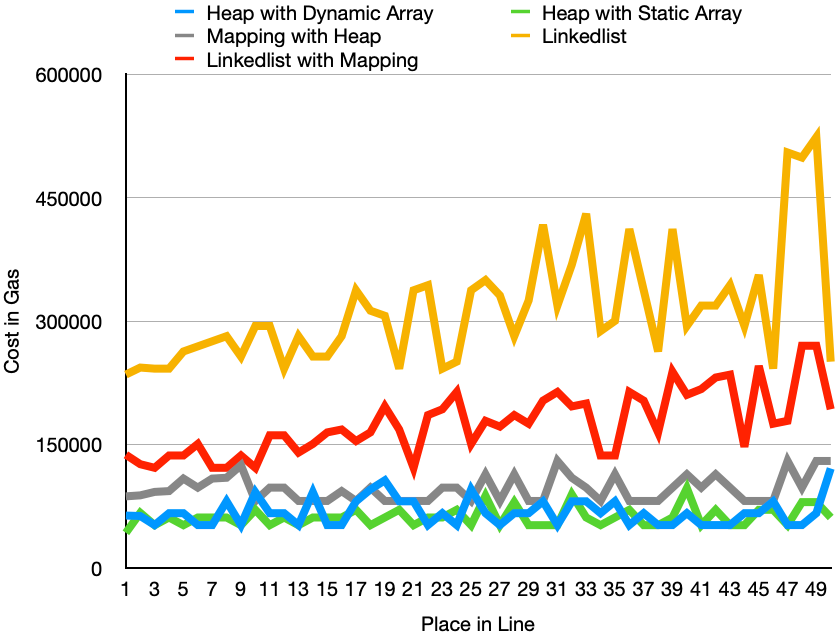
\includegraphics[width=1\textwidth]{fig/average_uints_insertion.png}
\caption{\footnotesize{}  \label{fig:average_uints_insertion}}
\end{figure}

% = = = = = = = = = = = = = = = = = = = = = = = = = = = = = = = = = = = = = = = =  %

Then, we call the \texttt{Dequeue()} function which iteratively removes the maximum value of the priority queue (until the data structure is empty). The computational costs for dequeuing 50 unsigned integers in each priority queue are outlined in Table~\ref{tab:PQ_UnitTests}. The tests are performed using the current Ethereum gas metrics (block gas limit $=$11,741,495 and 1 gas $=$ 56 gwei)~\footnote{https://ethstats.net/}. The second column of the table shows the net gas consumption (the gasUsed value derived from transaction receipts) for removing 50 integers from each priority queues.  

At the time of this writing, Ethereum transaction receipts only contain the net gas consumption and not the total gas consumption ( total gas consumption is defined as $gas refunded + gasUsed$ ) and we cannot find out the value of the EVM's refund counter from inside the EVM.

So in order to account for refunds inside each priority queue smart contract, we can calculate them manually; first we figure out exactly how much storage is being cleared when dequeuing  the max integers and then we could multiply the number of storage slots cleared by 15,000 (see the last column of Table~\ref{tab:PQ_UnitTests}).

Another way to know the amount of refund in each priority queue is to use \texttt{the estimateGas API} which provides a rough idea about the total amount of gas that is required for a transaction to go through. The \texttt{web3.eth.estimateGas} pretends the transaction is included in the block  and its functions (with the parameters passed) will be executed on the Ethereum blockchain. Doing so, it provides us an estimate of how much gas is needed to be sent with the transaction. The second and third columns of Table~\ref{tab:PQ_UnitTests}) show the total amount of gas required for dequeuing 50 integers from each priority queue (provided by estimateGas) as well as the amount of gas refund ($Total Gas Consumption - gasUsed$). 

Note that in order to urge miners to process smart contract with refunds, the accumulated gas refund can never exceed half the gas used up during computation~\cite{wood2014ethereum}. For example, the amount of gas that has been used when dequeuing 50 integers from the linkedlist with mapping data structure is 731,514 and since $3,000,000 > 731,514/2$, the accumulated refund through the transaction will be $731,514/2 = 365,757$.

% = = = = = = = = = = = =Uint testing the PQs Table = = = = = = = = = = = = =  %

\begin{table}[]
\centering
\begin{tabular}{|c|c|c|c|c|}
\hline

\textbf{\thead{Priority Queue}}    & \textbf{\thead{Net Cost\\in Gas}}      & \textbf{\thead{Total Cost\\in Gas\\(from estimateGas)}}      & \textbf{\thead{Gas Refund \\(from \texttt{estimateGas})}}    & \textbf{\thead{Gas Refund \\(Manually Calculated)}} \\ \hline

% = = = = = = = = = = = = = = = = = = = = = = = = = = = = = = = = = = = = = = = = = = = = = = = = = = = = = = = = = = = = = = = = = = = = = = %
	\textbf{\thead{Heap with \\ Dynamic Array}}         				& 2,547,031               & 3,312,378		& 765,347             & 750,000                       \\ \hline
% = = = = = = = = = = = = = = = = = = = = = = = = = = = = = = = = = = = = = = = = = = = = = = = = = = = = = = = = = = = = = = = = = = = = = = %
	\textbf{\thead{Heap with \\ Static Array}}           				& 1,324,856                & 2,090,182     	& 765,326             & 750,000                      \\ \hline
% = = = = = = = = = = = = = = = = = = = = = = = = = = = = = = = = = = = = = = = = = = = = = = = = = = = = = = = = = = = = = = = = = = = = = = %
	\textbf{\thead{Mapping with \\ keys stored \\ in Heap}} 		& 2,863,239                & 4,378,584       	& 1,515,345           & 1,500,000                     \\ \hline
% = = = = = = = = = = = = = = = = = = = = = = = = = = = = = = = = = = = = = = = = = = = = = = = = = = = = = = = = = = = = = = = = = = = = = = %
	\textbf{Linkedlist}                       							& 557,085               	& 1,772,085      	& 1,215,000           & 1,200,000                      \\ \hline
% = = = = = = = = = = = = = = = = = = = = = = = = = = = = = = = = = = = = = = = = = = = = = = = = = = = = = = = = = = = = = = = = = = = = = = %
	\textbf{\thead{Linkedlist with \\ Mapping}}          				& 731,514              	& 3,731,514       	& 3,000,000     	  &  3,765,000                       \\ \hline
% = = = = = = = = = = = = = = = = = = = = = = = = = = = = = = = = = = = = = = = = = = = = = = = = = = = = = = = = = = = = = = = = = = = = = = %

\end{tabular}
\caption{\footnotesize{}
\label{tab:PQ_UnitTests}}
\end{table}
% = = = = = = = = = = = = = = = = = = = = = = = = = = = = = = = = = = = = =  %



%============= Experiments =================== %
\section{Experiments}

Our application was developed in Solidity using the Truffle development framework and deployed on Ganache-CLI. We used Javascript for testing by leveraging the Mocha testing framework. Followings outline the results of different tests we performed.

%============= Test 1 (17_Worst_Case_Matching_test.js) Tables=================== %

 \subsection{Experiments on the \texttt{Match()} Function}

We executed the same test on the the five different versions of the CallMarket we implemented using five priority queues to examine the cost of the \texttt{Match()} function as well as the maximum pairs of bid and ask orders it can handle in each case. The \texttt{Match()} function's computational cost and the maximum number of orders it can execute in each case (before running out of gas) are outlined in Table~\ref{tab:worst_case_matching}. Note that this is a \textit{worst case matching} test where all bids and asks are submitted as marketable limit orders with specified prices that would be filled undoubtedly, performed using the current Ethereum gas metrics (block gas limit $=$11,741,495 and 1 gas $=$ 56 gwei)~\footnote{https://ethstats.net/}. The last column of Table~\ref{tab:worst_case_matching} shows the gas cost of matching 1000 pairs of bids and asks for each priority queue for which we set the block gas limit to the maximum of  $2^{53}$ (the Javascript's max safe integer).


%======= estimateGas() function = gasUsed + gasRefund =======%

% Heap with Dynamic Array: match.estimateGas() = 7204994 => gasRefund = 7204994 - 3274994 = 3930000
% Heap with Static Array: match.estimateGas() = 7337527 => gasRefund = 7337527 - 3107527 = 4230000
% Mapping with keys stored in Heap: match.estimateGas() = 6644803 => gasRefund = 6644803 - 5414803 = 1230000
% Linkedlist: match.estimateGas() = 7629847 => gasRefund = 7629847 -  3279847 = 4350000
% Linkedlist with Mapping: match.estimateGas() = 7227717 => gasRefund = 7227717 -  3297717 = 3930000

%===============================================%


% = = = = = = = = = = = =Worst_Case_Matching Table = = = = = = = = = = = = =  %

\begin{table}[]
\centering
\begin{tabular}{|c|c|c|c|}
\hline

\textbf{\thead{Priority Queue}}    & \textbf{\thead{Maximum Number \\ of \\ Matched Orders}}      & \textbf{\thead{Net Cost\\in Gas}}          & \textbf{\thead{Net Cost in Gas\\ for \\ 1000 Pairs \\ of Orders}} \\ \hline

% = = = = = = = = = = = = = = = = = = = = = = = = = = = = = = = = = = = = = = = = = = = = = = = = = = = = = = = = = = = = = = = = = = = = = = %
	\textbf{\thead{Heap with \\ Dynamic Array}}         				& 26 pairs                & 3,274,994                   	& 457,326,935                      \\ \hline
% = = = = = = = = = = = = = = = = = = = = = = = = = = = = = = = = = = = = = = = = = = = = = = = = = = = = = = = = = = = = = = = = = = = = = = %
	\textbf{\thead{Heap with \\ Static Array}}           				& 28 pairs                & 3,107,527                  	& 333,656,805                       \\ \hline
% = = = = = = = = = = = = = = = = = = = = = = = = = = = = = = = = = = = = = = = = = = = = = = = = = = = = = = = = = = = = = = = = = = = = = = %
	\textbf{\thead{Mapping with \\ keys stored \\ in Heap}} 		& 40 pairs                & 5,414,803                     & 319,481,722                       \\ \hline
% = = = = = = = = = = = = = = = = = = = = = = = = = = = = = = = = = = = = = = = = = = = = = = = = = = = = = = = = = = = = = = = = = = = = = = %
	\textbf{Linkedlist}                       							& 90 pairs                & 3,279,847                      & 35,823,601                        	\\ \hline
% = = = = = = = = = = = = = = = = = = = = = = = = = = = = = = = = = = = = = = = = = = = = = = = = = = = = = = = = = = = = = = = = = = = = = = %
	\textbf{\thead{Linkedlist with \\ Mapping}}          				& 130 pairs              & 3,297,717                       & 25,095,370                        \\ \hline
% = = = = = = = = = = = = = = = = = = = = = = = = = = = = = = = = = = = = = = = = = = = = = = = = = = = = = = = = = = = = = = = = = = = = = = %

\end{tabular}
\caption{\footnotesize{}
\label{tab:worst_case_matching}}
\end{table}



%%============= Test 3 (17_Worst_Case_Submission_test.js) Figures==================== %
%
% \subsection{Experiments on \texttt{Submit Order()} Functions}
%
%We executed another set of tests on the the five different versions of the CallMarket in which we sent 200 \texttt{SubmitBid} to the CallMarket to simulate two hundred of traders participating in the market. These tests were performed in two levels (i) worst case and (ii) average case submissions. 
%%the data structure used for bids and asks is the same and hence the submission plots for 200 submitbids and 200 submitasks. Do we have to mention that here?
%
%% = = = = = = = = = = = =Worst_Case_Submission = = = = = = = = = = = = =  %
%
%\subsubsection{Worst Case Order Submission}
%
%Here each \texttt{SubmitBid()} transaction has a price that is smallest or second-smallest of the transactions after it. Doing so, we ensure all the orders move every time a new order is sent to the market. Figure~\ref{fig:worst_case_submission} shows the gas cost variations for submitting 200 orders in five versions of the CallMarket. The x-axis is the place in line (\eg the 10th person to submit the order) and the and y-axis is the gas cost for sending that transaction.
%
%%And conversely each \texttt{SubmitAsk()} transaction has a price that is biggest or second-biggest of the transactions after it
%
%% = = = = = = = = = = = =Worst_Case_Submission Figure = = = = = = = = = = = = =  %
%
%\begin{figure}[htb!p]
%\centering
%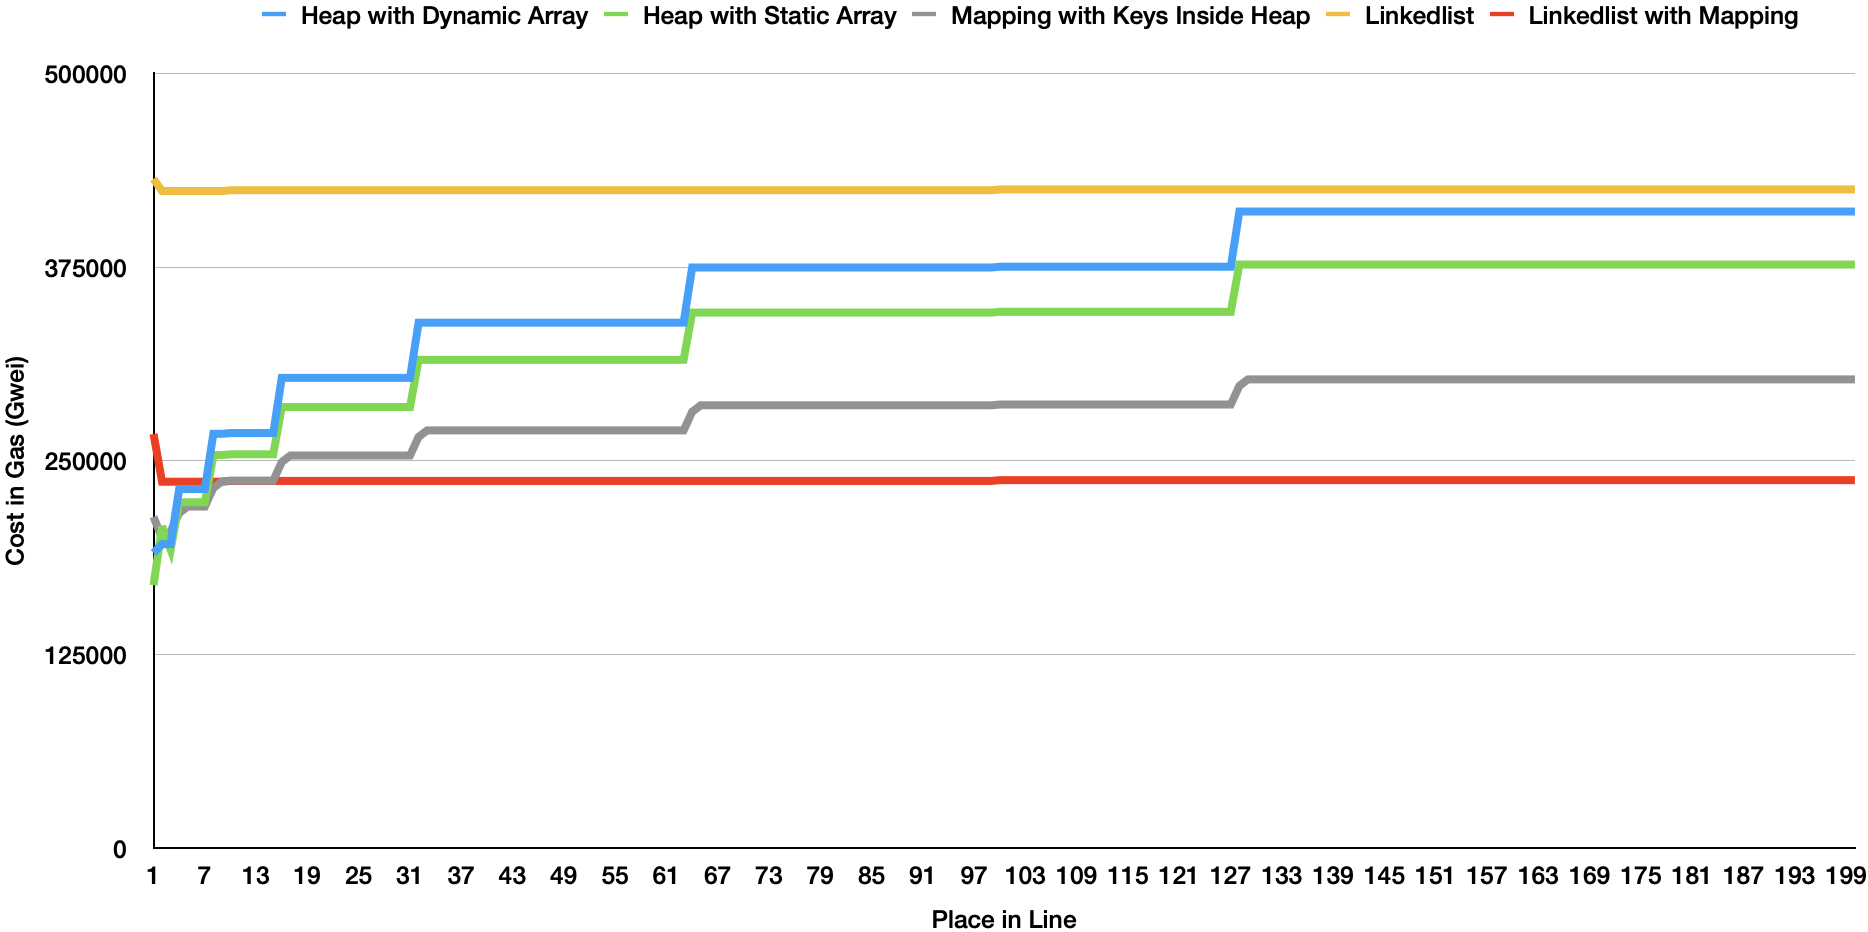
\includegraphics[width=1\textwidth]{fig/worst_case_submission_3.png}
%\caption{\footnotesize{}  \label{fig:worst_case_submission}}
%\end{figure}
%
%% = = = = = = = = = = = = = = = = = = = = = = = = = = = = = = = = = = = = = = = =  %
%
%
%% = = = = = = = = = = = =Average_Case_Submission = = = = = = = = = = = = =  %
%
%\subsubsection{Average Case Order Submission}
%
%Here we test the five versions of the CallMarket when 200 bid orders are entered in random ordering. To do so, we use JavaScript \texttt{Math.random()} function to generate pseudo-random integers between 1 and 100. Figure~\ref{fig:average_case_submission} shows the gas cost variations for submitting 200 orders in five versions of the CallMarket. Again the x-axis is the place in line (\eg the10th person to submit the order) and the and y-axis is the gas cost for submitting that transaction. 
%
%% = = = = = = = = = = = =Average_Case_Submission Figure = = = = = = = = = = = = =  %
%
%\begin{figure}[htb!p]
%\centering
%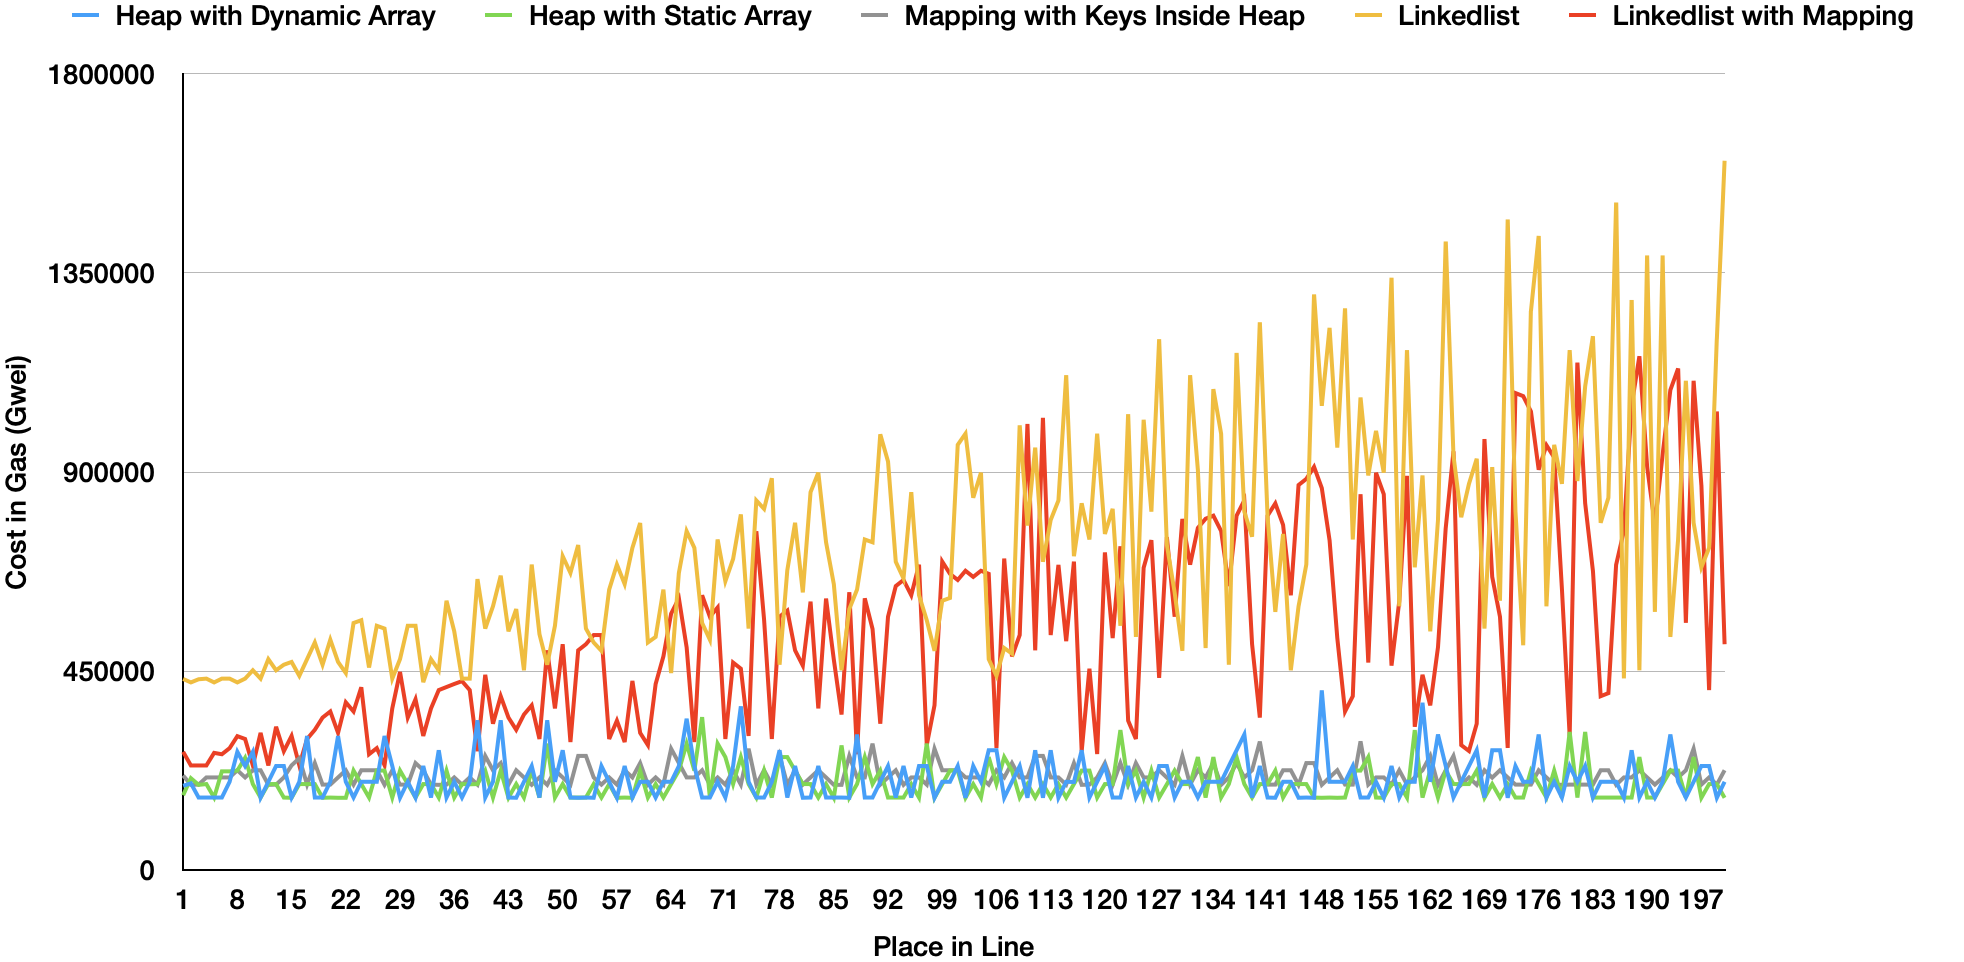
\includegraphics[width=1\textwidth]{fig/average_case_submission_3.png}
%\caption{\footnotesize{}  \label{fig:average_case_submission}}
%\end{figure}
%
%% = = = = = = = = = = = = = = = = = = = = = = = = = = = = = = = = = = = = = = = =  %














%======================================== %

% = = = = = = = = = = = = = = = = = = = = = = = = = = = = = = = = = = = = = = = = = =

\section{Concluding Remarks}


 
%\subsubsection*{Acknowledgements.} J. Clark thanks ...

































